\documentclass[8pt,aspectratio=169]{beamer}
\usetheme{Madrid}
\usepackage{graphicx}
\usepackage{booktabs}
\usepackage{adjustbox}
\usepackage{multicol}
\usepackage{amsmath}
\usepackage{amssymb}
\usepackage{tikz}
\usepackage{hyperref}
\usepackage{algorithm}
\usepackage{algorithmic}
\usepackage{colortbl}
\usepackage{pgfplots}
\pgfplotsset{compat=1.18}

% TikZ libraries for comics, diagrams, stakeholder maps
\usetikzlibrary{arrows.meta,positioning,shapes.callouts,shapes.geometric,decorations.pathreplacing}

% Color definitions
\definecolor{mlblue}{RGB}{0,102,204}
\definecolor{mlpurple}{RGB}{51,51,178}
\definecolor{mllavender}{RGB}{173,173,224}
\definecolor{mllavender2}{RGB}{193,193,232}
\definecolor{mllavender3}{RGB}{204,204,235}
\definecolor{mllavender4}{RGB}{214,214,239}
\definecolor{mlorange}{RGB}{255, 127, 14}
\definecolor{mlgreen}{RGB}{44, 160, 44}
\definecolor{mlred}{RGB}{214, 39, 40}
\definecolor{mlgray}{RGB}{127, 127, 127}
\definecolor{lightgray}{RGB}{240, 240, 240}
\definecolor{midgray}{RGB}{180, 180, 180}

% NEW COLORS for mini-lecture
\definecolor{dfteal}{RGB}{0,128,128}
\definecolor{dfred}{RGB}{180,30,30}

% Backward compatibility
\colorlet{MLPurple}{mlpurple}
\colorlet{MLBlue}{mlblue}
\colorlet{MLOrange}{mlorange}
\colorlet{MLGreen}{mlgreen}
\colorlet{MLRed}{mlred}
\colorlet{MLLavender}{mllavender}
\colorlet{MLGray}{mlgray}

% Theme colors (exact Madrid settings)
\setbeamercolor{palette primary}{bg=mllavender3,fg=mlpurple}
\setbeamercolor{palette secondary}{bg=mllavender2,fg=mlpurple}
\setbeamercolor{palette tertiary}{bg=mllavender,fg=white}
\setbeamercolor{palette quaternary}{bg=mlpurple,fg=white}
\setbeamercolor{structure}{fg=mlpurple}
\setbeamercolor{section in toc}{fg=mlpurple}
\setbeamercolor{subsection in toc}{fg=mlblue}
\setbeamercolor{title}{fg=mlpurple}
\setbeamercolor{frametitle}{fg=mlpurple,bg=mllavender3}
\setbeamercolor{block title}{bg=mllavender2,fg=mlpurple}
\setbeamercolor{block body}{bg=mllavender4,fg=black}
\setbeamertemplate{navigation symbols}{}
\setbeamertemplate{itemize items}[circle]
\setbeamertemplate{enumerate items}[default]
\setbeamersize{text margin left=5mm,text margin right=5mm}

% Footer
\setbeamertemplate{footline}{
  \leavevmode%
  \hbox{%
    \begin{beamercolorbox}[wd=.333333\paperwidth,ht=2.25ex,dp=1ex,center]{author in head/foot}%
      \usebeamerfont{author in head/foot}Methods and Algorithms
    \end{beamercolorbox}%
    \begin{beamercolorbox}[wd=.333333\paperwidth,ht=2.25ex,dp=1ex,center]{title in head/foot}%
      \usebeamerfont{title in head/foot}MSc Data Science
    \end{beamercolorbox}%
    \begin{beamercolorbox}[wd=.333333\paperwidth,ht=2.25ex,dp=1ex,right]{date in head/foot}%
      \usebeamerfont{date in head/foot}\insertframenumber{} / \inserttotalframenumber\hspace*{2ex}
    \end{beamercolorbox}}%
  \vskip0pt%
}

\newcommand{\bottomnote}[1]{%
\vfill
\vspace{-2mm}
\textcolor{mllavender2}{\rule{\textwidth}{0.4pt}}
\vspace{1mm}
\footnotesize
\textbf{#1}
}

\newenvironment{compactlist}{%
  \begin{itemize}%
    \setlength{\itemsep}{2pt}%
    \setlength{\parskip}{0pt}%
    \setlength{\parsep}{0pt}%
}{%
  \end{itemize}%
}

\newcommand{\highlight}[1]{\textcolor{mlorange}{\textbf{#1}}}
\newcommand{\mathbold}[1]{\boldsymbol{#1}}

% ============================================================
\title[Linear Algebra Mini-Lecture]{Linear Algebra for Machine Learning}
\subtitle{Mini-Lecture: The Mathematical Foundation}
\author{Methods and Algorithms}
\institute{MSc Data Science}
\date{}

\begin{document}

% ----------------------------------------------------------
% Slide 1: Title
% ----------------------------------------------------------
\begin{frame}[plain]
\vfill
\titlepage
\vfill
\end{frame}

% ----------------------------------------------------------
% Slide 2: XKCD Opening
% ----------------------------------------------------------
\begin{frame}{The ML Recipe}
\centering
\includegraphics[height=0.65\textheight]{images/1838_machine_learning.png}

\bottomnote{XKCD \#1838 by Randall Munroe (CC BY-NC 2.5)}
\end{frame}

% ----------------------------------------------------------
% Slide 3: Vectors
% ----------------------------------------------------------
\begin{frame}{Vectors: Direction and Magnitude}
\begin{columns}[T]
\begin{column}{0.55\textwidth}
\begin{compactlist}
\item A \highlight{vector} $\mathbf{x} \in \mathbb{R}^n$ represents one data point ---
      e.g.\ a loan applicant: $[\text{income},\;\text{age},\;\text{debt\_ratio},\;\text{credit\_score}]$
\item \highlight{Dot product} $\mathbf{a}^\top\mathbf{b} = \sum_i a_i b_i$ measures similarity between two feature vectors
\item \highlight{Norm} $\|\mathbf{x}\| = \sqrt{\mathbf{x}^\top\mathbf{x}}$ measures magnitude --- large norm $=$ extreme observation
\end{compactlist}
\end{column}
\begin{column}{0.42\textwidth}
\centering
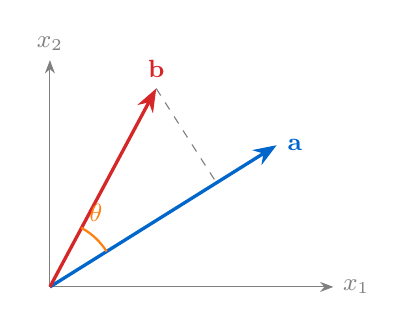
\begin{tikzpicture}[scale=0.9, >=Stealth]
  \draw[->,mlgray] (0,0) -- (4,0) node[right]{\small $x_1$};
  \draw[->,mlgray] (0,0) -- (0,3.2) node[above]{\small $x_2$};
  \draw[->,mlblue,very thick] (0,0) -- (3.2,2.0) node[right]{\small $\mathbf{a}$};
  \draw[->,mlred,very thick]  (0,0) -- (1.5,2.8) node[above]{\small $\mathbf{b}$};
  % angle arc
  \draw[mlorange,thick] (0.8,0.5) arc[start angle=32,end angle=62,radius=0.95];
  \node[mlorange] at (0.65,1.05) {\small $\theta$};
  % projection
  \draw[dashed,mlgray] (1.5,2.8) -- (2.35,1.47);
\end{tikzpicture}
\end{column}
\end{columns}

\bottomnote{Every ML algorithm starts with data encoded as vectors --- master this representation.}
\end{frame}

% ----------------------------------------------------------
% Slide 4: Matrices
% ----------------------------------------------------------
\begin{frame}{Matrices: Data as a Table}
\begin{compactlist}
\item The \highlight{design matrix} $\mathbf{X} \in \mathbb{R}^{n \times p}$: $n$ observations (rows), $p$ features (columns)
\item Each row is one customer; each column is one attribute (income, age, \ldots)
\item Matrix--vector product computes \highlight{all predictions at once}:
\end{compactlist}

\vspace{2mm}
\[
\hat{\mathbf{y}} \;=\; \mathbf{X}\,\boldsymbol{\beta}
\;=\;
\begin{pmatrix}
x_{11} & \cdots & x_{1p}\\
\vdots & \ddots & \vdots\\
x_{n1} & \cdots & x_{np}
\end{pmatrix}
\begin{pmatrix}\beta_1\\\vdots\\\beta_p\end{pmatrix}
\]
\vspace{1mm}

\begin{compactlist}
\item Finance example: 500 stocks $\times$ 10 factors $\Rightarrow$ \highlight{factor exposure matrix}
\end{compactlist}

\bottomnote{Think of $\mathbf{X}\boldsymbol{\beta}$ as ``apply the model to every observation simultaneously.''}
\end{frame}

% ----------------------------------------------------------
% Slide 5: Key Matrix Operations
% ----------------------------------------------------------
\begin{frame}{Key Matrix Operations}
\begin{compactlist}
\item \highlight{Transpose} $\mathbf{A}^\top$: flips rows and columns --- needed for $\mathbf{X}^\top\mathbf{X}$
\item \highlight{Inverse} $\mathbf{A}^{-1}$: ``undo'' a transformation --- $\mathbf{A}\mathbf{A}^{-1}=\mathbf{I}$
\item The product $\mathbf{X}^\top\mathbf{X}$ is covariance-like and powers the OLS solution (derived in L01)
\item $\det(\mathbf{A})=0$ means \highlight{singular} --- no unique inverse, features are linearly dependent
\end{compactlist}

\vspace{3mm}
\begin{block}{OLS Normal Equation (Preview)}
\[
\hat{\boldsymbol{\beta}} = (\mathbf{X}^\top\mathbf{X})^{-1}\mathbf{X}^\top\mathbf{y}
\]
\end{block}

\bottomnote{$\mathbf{X}^\top\mathbf{X}$ is the single most important matrix product in regression --- you will see it in L01.}
\end{frame}

% ----------------------------------------------------------
% Slide 6: Eigenvalues and Eigenvectors
% ----------------------------------------------------------
\begin{frame}{Eigenvalues and Eigenvectors}
\begin{columns}[T]
\begin{column}{0.55\textwidth}
\begin{compactlist}
\item \highlight{Eigen-equation}: $\mathbf{A}\mathbf{v} = \lambda\mathbf{v}$
\item $\lambda$ (eigenvalue) = \emph{how much} the vector is stretched
\item $\mathbf{v}$ (eigenvector) = \emph{which direction} stays unchanged
\item PCA uses eigenvectors of $\boldsymbol{\Sigma}$ to find principal components (details in L05)
\end{compactlist}

\vspace{2mm}
\begin{block}{Finance Insight}
Eigenvalues of a correlation matrix reveal independent \highlight{risk factors} --- large $\lambda$ = large variance explained.
\end{block}
\end{column}
\begin{column}{0.42\textwidth}
\centering
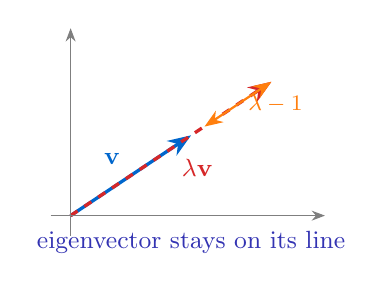
\begin{tikzpicture}[scale=0.85, >=Stealth]
  % original vector
  \draw[->,mlblue,very thick] (0,0) -- (1.8,1.2) node[midway,above left]{\small $\mathbf{v}$};
  % transformed vector (same direction, scaled)
  \draw[->,mlred,very thick,dashed] (0,0) -- (3.0,2.0)
        node[midway,below right]{\small $\lambda\mathbf{v}$};
  % annotation
  \draw[<->,mlorange,thick] (2.0,1.33) -- (3.0,2.0)
        node[midway,right]{\footnotesize $\lambda-1$};
  % axes
  \draw[->,mlgray] (-0.3,0) -- (3.8,0);
  \draw[->,mlgray] (0,-0.3) -- (0,2.8);
  \node[mlpurple,font=\small] at (1.8,-0.4) {eigenvector stays on its line};
\end{tikzpicture}
\end{column}
\end{columns}

\bottomnote{Eigenvectors point where data varies most --- PCA ranks them by eigenvalue magnitude.}
\end{frame}

% ----------------------------------------------------------
% Slide 7: Linear Transformations
% ----------------------------------------------------------
\begin{frame}{Linear Transformations}
\begin{compactlist}
\item \highlight{Matrix multiplication} = linear transformation of the input space
\item $\hat{\mathbf{y}} = \mathbf{X}\boldsymbol{\beta}$ transforms the feature space into a prediction space
\item \highlight{Rank} of $\mathbf{X}$ = number of linearly independent columns
\item If $\text{rank}(\mathbf{X}) < p$: \highlight{multicollinearity} --- OLS becomes unstable
\end{compactlist}

\vspace{3mm}
\begin{block}{Practical Check}
\[
\text{rank}(\mathbf{X}) = p \;\;\Longleftrightarrow\;\; \mathbf{X}^\top\mathbf{X} \text{ is invertible}
\;\;\Longleftrightarrow\;\; \text{unique OLS solution exists}
\]
\end{block}

\bottomnote{Multicollinearity is the \#1 numerical pitfall in linear regression --- regularization (L01) fixes it.}
\end{frame}

% ----------------------------------------------------------
% Slide 8: Norms and Distance Metrics
% ----------------------------------------------------------
\begin{frame}{Norms and Distance Metrics}
\begin{columns}[T]
\begin{column}{0.55\textwidth}
\begin{compactlist}
\item \highlight{L2 norm} (Euclidean): $\|\mathbf{x}\|_2 = \sqrt{\sum x_i^2}$ --- used in Ridge regression
\item \highlight{L1 norm} (Manhattan): $\|\mathbf{x}\|_1 = \sum |x_i|$ --- used in Lasso (sparse solutions)
\item Frobenius norm for matrices: $\|\mathbf{A}\|_F = \sqrt{\sum_{ij} a_{ij}^2}$
\item Finance: tracking error = $\|\mathbf{r}_{\text{port}} - \mathbf{r}_{\text{bench}}\|_2$
\end{compactlist}
\end{column}
\begin{column}{0.42\textwidth}
\centering
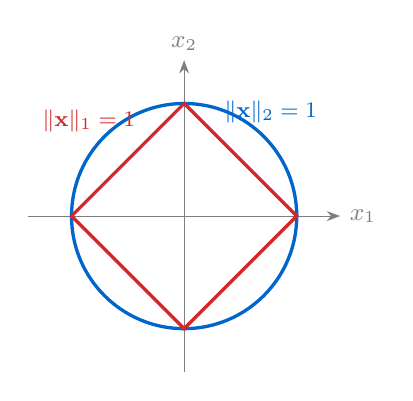
\begin{tikzpicture}[scale=1.1, >=Stealth]
  \draw[->,mlgray] (-1.8,0) -- (1.8,0) node[right]{\small $x_1$};
  \draw[->,mlgray] (0,-1.8) -- (0,1.8) node[above]{\small $x_2$};
  % L2 circle
  \draw[mlblue,very thick] (0,0) circle(1.3);
  \node[mlblue,font=\footnotesize] at (1.0,1.2) {$\|\mathbf{x}\|_2=1$};
  % L1 diamond
  \draw[mlred,very thick] (1.3,0) -- (0,1.3) -- (-1.3,0) -- (0,-1.3) -- cycle;
  \node[mlred,font=\footnotesize] at (-1.1,1.1) {$\|\mathbf{x}\|_1=1$};
\end{tikzpicture}
\end{column}
\end{columns}

\bottomnote{L1 produces sparse models (feature selection); L2 shrinks all coefficients evenly.}
\end{frame}

% ----------------------------------------------------------
% Slide 9: Covariance and Risk
% ----------------------------------------------------------
\begin{frame}{Finance: Covariance and Risk}
\begin{compactlist}
\item \highlight{Covariance matrix}: $\Sigma_{ij} = \text{Cov}(R_i, R_j)$ captures pairwise return co-movements
\item \highlight{Portfolio variance}: $\sigma_p^2 = \mathbf{w}^\top \boldsymbol{\Sigma}\, \mathbf{w}$, where $\mathbf{w}$ = asset weights
\item Eigendecomposition of $\boldsymbol{\Sigma}$ reveals independent \highlight{risk factors}
\end{compactlist}

\vspace{2mm}
\[
\boldsymbol{\Sigma} = \mathbf{V}\,\boldsymbol{\Lambda}\,\mathbf{V}^\top
\qquad\text{where}\quad
\boldsymbol{\Lambda} = \text{diag}(\lambda_1,\ldots,\lambda_p)
\]
\vspace{1mm}

\begin{compactlist}
\item \highlight{Cholesky decomposition} $\boldsymbol{\Sigma}=\mathbf{L}\mathbf{L}^\top$ generates correlated Monte Carlo samples
\end{compactlist}

\bottomnote{Nearly every risk model in quantitative finance starts with $\boldsymbol{\Sigma}$ and its eigenstructure.}
\end{frame}

% ----------------------------------------------------------
% Slide 10: Summary
% ----------------------------------------------------------
\begin{frame}{Summary: Linear Algebra Toolkit for ML}
\begin{enumerate}
\setlength{\itemsep}{6pt}
\item \highlight{Vectors} are data points; \highlight{matrices} are datasets --- $\mathbf{X} \in \mathbb{R}^{n\times p}$
\item $\mathbf{X}^\top\mathbf{X}$ powers the OLS solution and appears throughout regression (L01)
\item \highlight{Eigendecomposition} reveals variance directions --- foundation of PCA (L05)
\item \highlight{Norms} (L1, L2) drive regularization and distance-based methods (L01, L03)
\end{enumerate}

\vspace{4mm}
\begin{block}{Coming Up}
P02: Supervised \& Unsupervised Learning --- the two paradigms that organize this entire course.
\end{block}

\bottomnote{These four ideas --- vectors, $\mathbf{X}^\top\mathbf{X}$, eigenvalues, norms --- recur in every lecture.}
\end{frame}

\end{document}
